%==================================================================
% Ini adalah bab 3
% Silahkan edit sesuai kebutuhan, baik menambah atau mengurangi \section, \subsection
%==================================================================

\chapter[KONSEP RANCANGAN / PRODUK / JASA / EVALUASI / PENGUJIAN]
{KONSEP RANCANGAN}
\section{Waktu dan Tempat}
Penerbangan dilakukan kurang lebih 2 semester sekitar pukul 10:00 - 15:30 WIB, kemudian untuk uji coba \textit{quadcopter} memerlukan area yang luas, berumput, serta jauh dari jangkauan anak-anak. Maka dari itu untuk dapat terlaksana penelitian dengan baik dan aman, penelitian dilakukan pada lapangan terbuka yang bernama Lapangan Sono Royo Kayen, Condongcatur, Kec. Depok, Kabupaten Sleman, Daerah Istimewa Yogyakarta 55281

\section{Model Penelitian}
Jenis penelitian yang digunakan dalam penelitian ini adalah RnD/Research and Development adalah suatu proses pengembangan perangkat pendidikan yang dilakukan melalui serangkaian riset yang menggunakan berbagai metode dalam suatu siklus yang melewati berbagai tahapan.  Pengertian pengembangan menurut\cite{okpatrioka2023research}, RnD merupakan suatu proses pengembangan perangkat pendidikan yang dilakukan melalui serangkaian riset yang menggunakan berbagai metode dalam suatu siklus yang melewati berbagai tahapan. Research and Development (RnD) adalah metode penelitian yang digunakan untuk menghasilkan produk tertentu, dan menguji keefektifan produk tersebut.  Berdasarkan definisi-definisi diatas dapat dijelaskan bahwa penelitian pengembangan adalah penelitian yang digunakan untuk menghasilkan produk tertentu, dan untuk menyempurnakan suatu produk yang sesuai dengan acuan dan kriteria dari produk yang dibuat sehingga menghasilkan produk yang baru melalui berbagai tahapan dan validasi atau pengujian.

Dalam penelitian ini model yang diterapkan yaitu model penelitian ADDIE. Model ini berisi 5 proses yaitu Analysis, Desain, Development, Implementation,
Evaluasiom (ADDIE). Model perancangan alat yang digunakan adalah prototype \textit{quadcopter} yang bertujuan agar dapat membaca \textit{landing pad} sesuai perintah yang telah di buat sebelumnya. Model dari pengembangan ADDIE digunakan karena dinilai lebih rasional dan lengkap\cite{satriawan2023model}. Berikut merupakan penjelasan dari tahapan yang akan digunakan \cref{fig:al}:

\begin{figure}[H]
	\centering
	\includegraphics[scale=0.8]{C:/Users/ACER/Downloads/Template-LaTeX-Tugas-Akhir-Sarjana-Terapan-UNY-main/gambar/al}
	\caption{Metode Penelitian}
	\label{fig:al}
\end{figure}

Model dari pengembangan ADDIE digunakan karena dinilai lebih rasional dan lengkap. Berikut merupakan penjelasan dari tahapan yang akan digunakan:
\subsection{Analysis}
Analisys Tahap pertama suatu penelitian adalah menganalisis guna mengembangkan suatu produk baru dari pengembangan tersebut tercipta model, metode, media, dan bahan ajar yang layak sesuai dengan pengembangan produk sebelumnya. Pengembangan suatu produk dapat diawali dari masalah yang sudah ada. Masalah tersebut dapat muncul dan terjadi karena produk yang ada saat ini kurang relevan dengan kebutuhan sasaran, lingkungan belajar, teknologi yang semakin berkembang, dan sebagainya.
\subsection{Design}
Design Tahap kedua melakukan desain dalam model peneltian yang mengembangkan ADDIE merupakan proses sistematik yang dimulai dengan merancang konsep dan konten dalam produk tersebut. Pembuatan desain petunjuk penerapan diupayakan tertulis secara rinci agar dapat di pahami oleh orang lain yang melihat desain tersebut. Pada tahap ini rancangan dari produk masih bersifat konseptual dan akan mendasari proses pengembangan tahap berikutnya.
\subsection{Development}
Deveploment Tahap ketiga merupakan Deveploment dalam pengembangan ADDIE berisi mengenai kegiatan serta rancangan produk yang telah dibuat terlebih dahulu. Pada tahap sebelumnya, telah disusun kerangka konsep penerapan produk baru. Kerangka yang masih menjadi konsep tersebut selanjutnya direalisasikan menjadi produk yang siap untuk digunakan. Pada tahap ini juga perlu dibuat instrumen untuk mengukur kinerja dari produk baru yang telah di buat.
\subsection{Implementation}
Implementiont Tahap keempat merupakan penerapan produk dalam pengembangan ADDIE dimaksudkan untuk memperoleh balasan atau umpan balik terhadap produk yang dikembangkan. Umpan balik awal dapat diperoleh dengan menanyakan beberapa hal yang berkaitan dengan tujuan pengembangan produk. Penerapan di fokuskan pada rancangan yang telah di bikin.
\subsection{Evaluation}
Tahap kelima pada penelitian pengembangan ADDIE dilakukan untuk memberi umpan balik atau evaluasi kepada pengguna produk, segingga rvisi dibuat sesuai dengan hasil evaluasi atau kebutuhan yang belum dapat terpenuhi oleh produk tersebut. Tujuan dari evaluasi akhir ini untuk mengukur ketercapaian dari pengembangan yang telah dilakukan.

\section{Analisis Kebutuhan}
Analisis kebutuhan adalah tahap awal penentuan topik penelitian dalam hal ini adalah pembacaan \textit{helipad}. Dari topik tersebut kemudian dapat menentukan komponen apa saja yang akan digunakan saat membangun prototype. Tidak hanya menentukan jenis komponen namun juga dapat membandingkan kualitas pada komponen yang akan digunakan saat penelitian berlangsung. Dalam tahap analisis terdapat 3 jenis yakni menganalisis kebutuhan hardware,software, dan elektronik yang akan di pakai.

\subsection{Hardware}
\begin{packed_item}
	\item [1.]\textit{Landing} skit
	berfungsi membantu proses pendaratan pada \textit{quadcopter}, \textit{landing} skit sebagai penopang pada \textit{quadcopte}r, sehingga komponen di atasnya tidak langsung menyentuh permukaan tanah jika komponen langsung menyentuh tanah maka sangat besar resiko terjadinya kerusakan.
	\item [2.] \textit{Frame Quadcopter}
	berfungsi sebagai wadah atau tempat pemansangan komponen elektronik. \textit{Frame} jenis F405 memiliki 4 sisi yang dapat digunakan sebagai tempat motor \textit{brushless} dipasang.
	\item [3.]Baut M2
	berfungsi untuk mengabungkan beberapa komponen elektronik dan menjadi satu bagian yang memiliki sifat tidak permanen atau dapat di lepas pasang  menggunakan obeng.
	\item [4.]\textit{Propeller}
	adalah salah satu komponen penting yang memiliki fungsi untuk memberikan daya angkat pada \textit{quadcopter}, pengendalian arah, serta penyeimbangan. \textit{Propeller} dapat berputas karena terdapat motor dibawahnya dari kerja tersebut menghasilkan gaya dorong yang dapat membuat quadcopter terbang.
	\item [5.]\textit{Damper}
	memiliki fungsi sebagai peredam saat guncangan terjadi, \textit{damper} di pasang pada empat titik kanan kiri bagian bawah \textit{flight controller}. Selain sebagai peredam dengan pemasangan damper juga dapat memaksimalkan pembacaan sensor yang berada di \textit{flight controlle}r.
	\item [6.]\textit{Stand}GPS
	berfungsi sebagai tempat GPS dipasang, letak stand GPS berada pada bagian atas \textit{quadcopter}.
\end{packed_item}

\subsection{Software}
\begin{packed_item}
	\item [1.]\textit{Mission Planner}
	adalah \textit{softwar}e yang menjadi stasiun \textit{control} darat untuk \textit{plane, copter, dan cover}. Di dalam \textit{software} ini terdapat berbagai fitur lengkap yang dapat digunakan untuk proyek \textit{autopilot}. Pada penelitian ini \textit{mission planner} digunakan sebagai \textit{software} yang dapat mengkonfigurasi FC mulai dari kalibrasi sensor hingga mengatur parameter seperti \textit{ARMING CHECK},PID dan lain lain.
	\item [2.]\textit PhyCharm
	adalah editor yang dapat digunakan selain IDLE, kelebihan nya lebih ringan serta praktik karena PhyCharm dibangun mengggunakan phyton, maka dukungan terhadap bahasa pemograman tersebut cukup lengkap. PyCharm mendukung beberapa perpustakaan, termasuk Matplotlib dan SciPy, yang membantu proyek ilmu data dan pembelajaran mesin. Fitur pemfaktoran ulang PyCharm membantu memperbaiki struktur program tanpa berdampak negatif pada kinerjanya. Pengguna dapat mengubah variabel lokal dan global dengan cepat dan global. Mereka juga dapat menggunakan metode ekstraksi untuk mengekstrak kelas dan fungsi yang luas. Ia juga memiliki banyak fitur lain seperti memperkenalkan konstanta atau variabel, \textit{pull up, pull down, dan rename}.
	\item [3.]\textit Honestech VHS to DVD 3.0 SE
	software ini digunakan untuk membaca dan memberikan tampilan desktop yang tersambung pada camera quadcopter. Honestech VHS to DVD 3.0 SE memiliki fitur rekam yang berfungsi untuk mengumpulkan data hasil percobaan membaca landing patch pada quadcopter.
	\item [4.]\textit BLHeli
	terdapat ESC yang dapat diprogram mulai dari karakteristik putaran, arah putaran, dan kecepatan motor. BLHeli dipilih karena penggunaannya yang mudah di pahami, serta fitur di dalamnya lengkap.
\end{packed_item}

\subsection{Elektronik}
\begin{packed_item}
	\item [1.]\textit{Flight Controller} PIXHAWK
	merupakan komponen utama dari otak penggerak yang dapat memberikan bantuan pada penerbangan \textit{quadcopter}. \textit{Flight Controller}(FC) merupakan perangkat yang akan menerima , memproses, dan mengeluarka data. Pada penelitian ini PIXHAWK dipilih karena installasi mudah. Flight controller diisi dengan fimware ardupilot yang dapat bekerja secara \textit{autonomous}.
	\item [2.]\textit ESC CYCLONE
	adalah komponen elektronik penghubung motor, baterai, dan \textit{controller} yang digunakan sebagai pengubah kecepatan motor sehingga dapat mengatur gerakan yang terjadi pada \textit{quadcopter}.
	\item [3.]\textit GPS
	berfungsi untuk memberikan posisi dan kecepatan mengenai \textit{quadcopter}. GPS(Global Positioning System) merupakan kunci pergerakan arah quadcopter agar dapat menjalankan berbagai misi penting yakni RTH\textit{(Return To Home)}, RTL\textit{(Return To Launch)}, dan mode terbang \textit{althold} serta \textit{poshold}. Pada penilitian ini menggunakan GPS versi M10Q karena mudah untuk di konfigurasi
	\item [4.]\textit{Flight Controller} PIXHAWK
	merupakan komponen akuator yang akan dapat mengkonfersikan tenaga listrik yang berasal dari baterai menjadi tenaga mekanik berupa putaran. Motor akan mengkonversi data dari ESC menjadi putaran, motor memiliki berbagai macam variasi putaran sesuai dengan perintah program yang dikimkan.
	\item [5.]\textit Radio \textit{Control}
	digunakan sebagai pemberi perintah ke FC melalui receiver untuk kemudian di salurkan sinyal nya ke ESC. Pada mode \textit{autonomous}, RC berfungsi sebagai pengaman \textit{quadcopter} apabila terjadi kesalahan pada pengiriman program.
	\item [6.]\textit Baterai
	berfungsi sebagai pemasok listrik utama ke sistem gerak, lampu lampu dan komponen kelistrikan lainnya pada \textit{quadcopter}. Pada penelitian ini digunakan baterai jenis 4S yang memiliki 4 \textit{cell} dimana tiap \textit{cell} memiliki tegangan konstan sebesar 3.75 Volt. Agar baterai tetap dalam tegangan konstan yang sesuai maka penggunaan nya harus hati hati agar tidak merubah tegangan pada baterai tersebut.
	\item [7.]\textit{Video}Receiver
	digunakan sebagai penerima data dari \textit{video}transimtter yang berupa \textit{video}. Pada \textit{video}receiver terdapat konfigurasi frekuensi dan \textit{channel} yang mana harus di ubah sedemikian rupa sehingga dapat terhubung dengan \textit{video} transmitter.
	\item [8.]\textit Kamera dan \textit{video} Transmiter
	digunakan sebagai mata untuk mendeteksi objek pada bagian bawah \textit{quadcopter}. Objek yang terdeteksi kemudian ditangkap dalam satuan detik, diteruskan oleh \textit{video} transmitter untuk diterima oleh \textit{video} reciver yang terpasang pada laptop atau \textit{ground control}. Pada \textit{video} transmitter terdapat konfigurasi channel yang nantinya akan disesuaikan dengan \textit{video} reciver agar dapat terhubung.
	\item [9.]\textit Telemetry 433MHz
	adalah perangkat elektronik yang berfungsi membaca data dan mengirimkan nya. Dalam hal \textit{quadcopter}, telemetry terbagi menjadi dua bagian yakni Ground dan Air. Pada  perangkat ground berfungsi menerima data dari perangkat air dan dapat mengirimkan kembali data tersebut ke perangkat air. Sedangkan pada perangkat air \textit{quadcopter} berfungsi mengirimkan data dari \textit{quadcopter }dan menerima data dari perangkat \textit{ground}.
\end{packed_item}

\section{Rancang Pengembangan Sistem}
\subsection{Desain Mekanik}
Desain \textit{quadcopter} yang digunakan pada penelitian ini adalah konfigurasi \textit{frame quadcopter} yaitu dengan menggunakan empat propeller dengan X \textit{frame} dan juga empat kaki sebagai tahanan wahana pada \textit{quadcopter} saat berada di atas permukaan tanah. Desain mekanik wahana menggunakan konfigurasi 4 motor BLDC membentuk sudut 45 derajat dengan sumbu X dan Y pada wahana. Berikut desain wahana \textit{quadcopter} yang digunakan pada penelitain ini, seperti ditunjukan pada \cref{fig:desain}.

\begin{figure}[H]
	\centering
	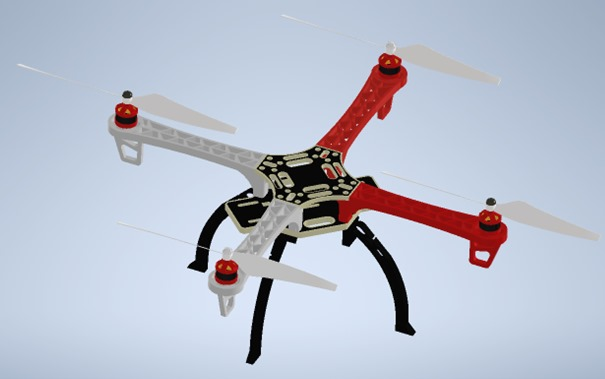
\includegraphics[scale=0.4]{C:/Users/ACER/Downloads/Template-LaTeX-Tugas-Akhir-Sarjana-Terapan-UNY-main/gambar/desain}
	\caption{Desain mekanik}
	\label{fig:desain}
\end{figure}

Fungsi \textit{webcam} sebagai sensor \textit{vision} pada penelitian ini adalah untuk mengambil citra rekaman udara dan mengirimkan data ke komputer vision. Sistem menghasilkan deteksi frame dengan nama dan presentase nilai \textit{confidance}.

\subsection{Desain Elektrikal Pendeteksian}
Komponen elektronik dipakai oleh \textit{flight controller} dengan kabel sebagai penghubung antar komponen. Perakitan khusus terletak pada komponen ESC, karena terdapat aturan pemasangan kabel yang akan menentukan putaran arah motor. ESC 1 hingga ESC 4 memiliki kabel data yang terpasang secara berurutan pada \textit{flight controller}. Pemasangan kabel ESC turut mempengaruhi konfigurasi jenis \textit{frame} yang digunakan dalam hal ini \textit{frame} X. Instalasi komponen digambarkan sebagai berikut \cref{fig:ds}.

\begin{figure}[H]
	\centering
	\includegraphics[scale=0.6]{C:/Users/ACER/Downloads/Template-LaTeX-Tugas-Akhir-Sarjana-Terapan-UNY-main/gambar/ds}
	\caption{Desain Elektrikal Pendeteksian}
	\label{fig:ds}
\end{figure}


\subsection{Perancangan Sistem Deteksi Landing Pad}
Landing pad yang digunakan berukuran diamater 25cm x 25cm ketebalan 3mm dengan huruf "H" di tengahnya, \cref{fig:lan} merupakan objek \textit{landing pad} yang akan di pakai dalam pengambilan dataset dan pengujian pada sistem deteksi kali ini.

\begin{figure}[H]
	\centering
	\includegraphics[scale=0.5 ]{C:/Users/ACER/Downloads/Template-LaTeX-Tugas-Akhir-Sarjana-Terapan-UNY-main/gambar/lan}
	\caption{Perancangan Sistem Deteksi Landing Pad}
	\label{fig:lan}
\end{figure}

Pada penelitian ini menggunakan bahasa Python dengan Google Colaboratory sebagai \textit{platfrom} pada komputer \textit{training}, vision yang digunakan yaitu kamera \textit{smartphone} yang telah terpasang pada prototipe yang terhubung dengan komputer vision. Program Python yang dibuat nantinya akan memuat algoritma YOLO yang kemudian akan memperoses citra dari input yang diperoleh dari kamera \textit{smartphone} secara \textit{real-time}. Algoritma YOLO akan membagi gambar menjadi grid dengan ukuran s x s. Kemudian di setiap grid akan memprediksi \textit{bounding box} dan peta klasifikasi untuk setiap kelas grid tersebut\cite{nazilly2020implementasi}. Setelah melalui proses oleh YOLO,layar monitor yang telah terhubung dengan komputer vision akan menampilkan \textit{display window} berupa \textit{frame} citra yang didalamnya terdapat objek deteksi dengan ditandai oleh \textit{bounding box} serta nilai \textit{confidance}.

\subsection{Implementasi Metode YOLO}
Desain deteksi objek berupa \textit{landing pad} menggunakan algoritma YOLO dapat dilihat dari \cref{fig:sistem-yolo}.

\begin{figure}[H]
	\centering
	\includegraphics[scale=0.8]{"C:/Users/ACER/Downloads/Template-LaTeX-Tugas-Akhir-Sarjana-Terapan-UNY-main/gambar/Sistem YOLO"}
	\caption{Desain sistem}
	\label{fig:sistem-yolo}
\end{figure}

Dari diagram alir diatas dapat ditunjukan beberapa tahap dalam penerapan nya dari mulai metode Darknet YOLO, diantaranya sebagai berikut ini. Pertama, pengambilan dataset, dilakukan pada ketinggian \textit{(altitude)} 1 meter, 2 meter,3 meter, 4 meter. Dan menggunakan resolusi 3032x2008 \textit{pixel} atau 6MP dengan kondisi cahaya sekitar pukul 10:00-15:30 WIB. Dataset yang digunakan berjumlah kurang lebih 1000 gambar, dengan rasio 80\% untuk \textit{training set} dan 20\% untuk \textit{validation set}. Dataset gambar yang telah terkumpul akan melalui proses label di setiap \textit{frame} gambar. Label dataset, merupakan proses penambahan informasi pada citra dalam dataset, pada penelitian ini menggunakan YOLO. Setiap gambar diberi label untuk mendapatkan koordinat \textit{bounding box} sesuai dengan keadaan sebenarnya \textit{(ground-truth bounding box)}, yang akan dibandingkan dengan \textit{bounding box} yang diprediski. Dengan perbandingan yang terjadi dari kedua jenis maka didaptkan nilai \textit{Intersection over Union}(IoU).

Langkah selanjutnya, \textit{training} atau pelatihan dilakukan menggunakan algoritma YOLO. Proses pelatihan menggunakan Google Colaboratory. Selama proses \textit{training}, \textit{hyperparameter} seperti \textit{learning rate} dan momentum dapat disesuaikan untuk meningkatkan konvergensi model. Evaluasi kinerna model dataset dapat membantu mengontrol \textit{overfitting} dan memastikan generalisasi yang baik. Iterasi di ullang hingga YOLO mencapai kinerja yang sesuai untuk deteksi objek lebih cepat serta akurat. 

Selah menyelesaikan tahap \textit{training} dataset, dilakukan pengujian sistem deteksi dengan menggunakan file \textit{weights} yang dihasilkan pada proses \textit{training} sebelumnya. Pengujian sistem ini dilaksakan secara \textit{offline} dengan cara memberikan \textit{input} gambar ke sistem deteksi. Hasil pengujian tersebut akan mencakup \textit{boundiing box} yang sesuai dengan koordinat (x, y, w, h), nilai \textit{confidance}, dan probabilitas atau peluang kelas dari objek yang terdeteksi.

\section{Rancang Uji Fungsi}
Perancangan uji sistem berfungsi untuk mengetahui fungsional dari setiap komponen\textit{quadcopter}. Rancangan uji sistem meliputi perencanaan pengujian elektronik dan pengujian \textit{software}.
\subsection{Uji Elektronik}
Pada Tahapan pengujian ini terdapat pengujian komponen elektronik yang sudah terkoneksi dengan hardware. Pengujian ini berfungsi untuk melihat koneksi antara hardware dan elektronik pada rangkaian \textit{quadcopter}. Hal tersebut dapat dilihat dari  \cref{tab:ujiel} berikut.


\begin{table}[h]
	\caption{Uji Elektronik}
	\label{tab:ujiel}
	\centering
	\begin{tabular}{|l|l|l|}
		\hline
		NO & Pengujian & Keterangan \\ \hline
		1 & GPS &  \\ \hline
		2 & Telemetry &  \\ \hline
		3 & Kamera Smartphone &  \\ \hline
		4 & Motor 1 &  \\ \hline
		5 & Motor 2 &  \\ \hline
		6 & Motor 3 &  \\ \hline
		7 & Motor 4 &  \\ \hline
		8 & Accelometer Level &  \\ \hline
		9 & Accelometer Right &  \\ \hline
		10 & Accelometer Left &  \\ \hline
		11 & Accelometer Nose Up &  \\ \hline
		12 & Accelometer Nose Down &  \\ \hline
		13 & Accelometer Back &  \\ \hline
	\end{tabular}
\end{table}

\subsection{Uji Software}
Rancangan uji \textit{software} meliputi rancangan pengujian program guna mengontrol pergerakan \textit{quadcoper}. Pengujian dilakukan menggunakan \textit{software} Pychram dengan memanfaatkan \textit{library} dronekit dengan menggunakan bahasa Python. Hal tersebut dapat dilihat \cref{tab:ujisof} berikut.

\begin{table}[h]
	\caption{Uji Software}
	\label{tab:ujisof}
	\centering
	\begin{tabular}{|l|l|l|l|}
		\hline
		NO & Pengujian & Hasil Uji Python & Hasil Uji Remote Control \\ \hline
		1 & Pitch &  &  \\ \hline
		2 & Roll &  &  \\ \hline
		3 & Yaw &  &  \\ \hline
		4 & Take Off &  &  \\ \hline
		5 & Landing &  &  \\ \hline
	\end{tabular}
\end{table}

Rancangan pengujian menggunakan remote memiliki tujuan untuk menguji kualitas terbang \textit{quadcopter} dan kualitas \textit{controlling} menggunakan remote. Sedangkan rancangan uji menggunakan program dari Pychram yang berfungsi guna melihat kesiapan pergerakan pada \textit{quadcopter}.

\section{Pengujian Deteksi \textit{Landing Pad}}
	Uji \textit{landing pad} ditunjukan untuk melihat kesiapan kualitas \textit{quadcopter} saat mengambil data guna \textit{landing}pada area yang di tentukan uji ini menggunakan kamera, \textit{remote control} atau secara otonom melalui program yang telah di \textit{setting} sebelumnya. Pengujian deteksi ditunjukan guna menyiapkan tinggi rendah kamera pada \textit{quadcopter} untuk menggambil data guna proses \textit{training} atau pelatihan pada jaringan YOLO menggunakan \textit{halipad}. Pengujian ini dilakukan dengan dua cara manual serta otonom. Hasil uji dapat ditulis ke \cref{tab:ujidek}
	
	\begin{table}[h]
		\caption{Uji Deteksi Landing Pad}
		\label{tab:ujidek}
		\centering
		\begin{tabular}{|l|l|l|l|}
			\hline
			NO & Jarak Kamera & Hasil Deteksi Otonom & Hasil Deteksi Manual \\ \hline
			1 & 50 cm &  &  \\ \hline
			2 & 100 cm &  &  \\ \hline
			3 & 150 cm &  &  \\ \hline
			4 & 200 cm &  &  \\ \hline
			5 & 250 cm &  &  \\ \hline
			6 & 300 cm &  &  \\ \hline
			7 & 350 cm &  &  \\ \hline
			8 & 400 cm &  &  \\ \hline
		\end{tabular}
	\end{table}
